\section{Model}

\subsection{Description}
\begin{figure}[h!]
    \centering
    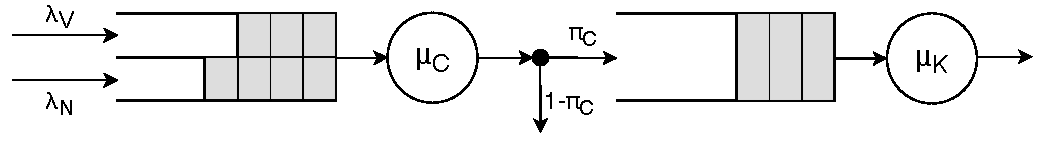
\includegraphics[width=.75\textwidth]{figs/qt_model.pdf}
    \caption{Schematic representation of the model of the bar.}
    \label{fig:model}
\end{figure}

In \cref{fig:model} you can see the model of the bar, where:
\begin{itemize}
    \item $\lambda_V$ is the average arrival rate for VIP customers;
    \item $\lambda_N$ is the average arrival rate for ``normal'' (i.e. non-VIP) customers;
    \item $\mu_C$ is the average service rate of the cashier ($r_{cashier}$);
    \item $\mu_K$ is the average service rate of the kitchen ($r_{kitchen}$);
    \item $\pi_C$ is the ratio of compound orders over the total, i.e. the 
        probability that an order is compound.
\end{itemize}

The cashier is modeled as a service center with two queues that are managed 
in an head-of-line-priority fashion.

The kitchen is modeled as a simple M/M/1 service center. Note that if VIP 
priority is introduced also in the kitchen, it will become identical to the 
cashier, mutatis mutandis.

\subsection{Assumptions}
The following assumptions were made when modeling the system:
\begin{itemize}
    \item No renegation: customers cannot leave the queue.
    \item No jockeying: VIP customers cannot move to the normal customers' queue.
    \item No overtaking: customers cannot change their position in queue.
    \item Infinite queuing space: there is no upper bound in the number of 
        customers in a queue.
    \item the inter-arrival times of VIP and normal customers are independent 
        RVs.
    \item the type of an order (simple or compound) is independent of the other
        orders.
    \item the service rate is the same for normal and VIP customers.
\end{itemize}

\subsection{Factors}
The factors that can affect the modeled system are:
\begin{itemize}
    \item cashier service rate: $\mu_C$
    \item kitchen service rate: $\mu_K$
    \item ratio of compound orders over the total: $\pi_C$ 
    \item average inter-arrival rate of VIP orders: $\lambda_V$
    \item average inter-arrival rate of Normal orders: $\lambda_N$
    \item Kitchen queue type: "FIFO" or "priority"
\end{itemize}

\subsection{Stochastic model for the exponential scenario}
In the exponential scenario, we can formulate a stochastic model of the system
using queuing theory.

The cashier priority queuing is, in fact, a well known queuing 
strategy (L. Kleinrock, 1976)\footnote{Leonard Kleinrock (1976). Head-of-the-Line Priorities.\emph{Queueing systems, volume 2: Computer applications} (pp. 119-126). New York, Wiley.}. In the case of two static priorities, the following equations for
the average waiting time hold:

\begin{align}
    E[W^C_{V}] &= \frac{\lambda_V + \lambda_N}{(\mu_C-\lambda_{V})\mu_C} \label{eq:waitvip}\\
    E[W^C_{N}] &= \frac{\lambda_V + \lambda_N}{(\mu_C-\lambda_{V}-\lambda_N)(\mu_C-\lambda_{V})} \label{eq:waitnorm}
\end{align}

Note that, for $\lambda_V = 0$ (or $\lambda_N = 0$) the above equations are the 
same as for an M/M/1 system.

In order to obtain the average response times, we just need to add $\frac{1}{\mu_C}$
due to the linearity of the mean operator.

Furthermore, note that if we didn't make any distinction between orders and just 
saw them entering the cashier SC and exiting it, we would not be able to 
distinguish it from an M/M/1 SC with arrival rate $\lambda_V + \lambda_N$ and 
service rate $\mu_C$ just by looking at the distribution of the 
inter-departure times (we don't care about the order).

This result has been confirmed by the validation runs on the simulator. 
Please note that this would not have hold if service rate were different between
normal and VIP customers.

Therefore, we can apply queueing network theory which tells us that the average 
arrival rate at the kitchen is the same as an M/M/1 SC with arrival rate equal 
to $\pi_C(\lambda_V+\lambda_N)$. Thus, the response time of the kitchen 
(independently of the customer type) is:

\begin{align}
    E[R^K] &= \frac{1}{\mu_K-\pi_C(\lambda_{V}+\lambda_{N})}
\end{align}

Please note that, if the kitchen had a priority queuing, we would not be able
to follow the same reasoning above. However, simulation results suggest that 
the mean waiting time could be computed as in \cref{eq:waitvip,eq:waitnorm}
considering $\pi_C \lambda_N$ and $\pi_C \lambda_V$ as the arrival rates.

Finally, we can write the average response times for the four classes of orders:
\begin{align}
    E[R_{N,S}] &= E[W^C_{N}] + \frac{1}{\mu_C} \\
    E[R_{N,C}] &= E[W^C_{N}] + \frac{1}{\mu_C} + E[R^K] \\
    E[R_{V,S}] &= E[W^C_{V}] + \frac{1}{\mu_C} \\
    E[R_{V,C}] &= E[W^C_{V}] + \frac{1}{\mu_C} + E[R^K]
\end{align}